\documentclass[11pt]{article}
\usepackage[utf8]{inputenc}

\usepackage{biblatex}
\bibliography{references}
\usepackage{amsmath}

\usepackage{algorithm}
\usepackage{algorithmic}
\usepackage{accents}
\usepackage{amsfonts}


\usepackage{xcolor}


\usepackage{multimedia}
\usepackage{graphicx}
\graphicspath{{./images/}}

\usepackage[section]{placeins}

\usepackage{float}

\newcommand{\states}{\mathcal{S}}
\newcommand{\actions}{\mathcal{A}}
\newcommand{\real}{\mathbb{R}}
\newcommand{\data}{\mathcal{D}}
\newcommand{\new}{\text{new}}
\newcommand{\old}{\text{old}}
\newcommand{\for}{\text{for}}
\newcommand{\argmax}[1]{\underset{#1}{\text{arg max }}}

\newcommand{\marek}[1]{\textcolor{red}{#1}}
\newcommand{\connor}[1]{\textcolor{green}{#1}}
\newcommand{\emma}[1]{\textcolor{blue}{#1}}

\usepackage[margin=1.1in]{geometry}

\title{Robust Probabilistic Imitation Learning}
\author{Brendan Crowe}
\date{December 2020}


\begin{document}

\maketitle

\begin{abstract}
    As Imitation Learning (IL) becomes a more popular area of research and its applications reach real world problems, the necessity to deal with adversarial data in a structured way grows. Most approaches as of now assume the data is perfect, no adversary. However, in real world applications this assumption can be detrimental. Being able to detect and remove adversarial demonstrations is paramount for the success of IL. This paper proposes a probabilistic approach to autonomously detect and re-weight adversarial demonstrations, as it learns a policy from the expert demonstrations. The problem posed in this work can then be elegantly solved using an Expectation Maximization (EM)-esque algorithm. The proposed method is statistically robust to adversarial demonstrations and thus will be titled Robust Probabilistic Imitation Learning (R-PIL). Furthermore, being probabilistic in nature, this could be used as a general method for re-weighting demonstrations in other frameworks.
\end{abstract}

\section{Introduction}

\quad Imitation Learning (IL) or learning a task from demonstrations, has many theoretical applications in robotics, control systems, etc. In recent years, IL has achieve great results in simulations and controlled experiments \cite{ho2016generative} \cite{ramachandran2007bayesian}. An assumption that many IL frameworks make today is that the demonstrations provided are completing the task in an optimal way, and that they are correct, not failed or corrupted. While this assumption is easy to verify in simulations and laboratory experiments, that may not be possible in the real world. When attempting to teach an agent (a robot or other device) to learn a task, the exact dynamics or optimal solution, may be unknown to the modeler. In this situation, it could be difficult or time consuming to determine if any of the demonstrations are following a non-optimal or downright incorrect strategy. An adversary in this context, is any agent (human or other) that is not following an optimal or safe policy for the task, where a policy being the way that one completes the task. These adversarial demonstrations can be detrimental to IL not only because they could prevent learning of the task, but because they could cause an agent to learn an unsafe way to approach the task.

Let us examine an example. We want to teach a self driving car by have experts (humans) show the car how to drive. Humans would drive the car and sensor embedded in the car would collect various features that could be used to train an autonomous agent. In this case, we could have several kinds of drivers that would be adversarial. There could be someone who is a poor drivers, reckless drives, or simply the sensors in the car could be corrupted. In the case of a self driving car, the car may be able to learn to drive despite adversarial demonstration, but it might learn unsafe behavior as a result e.g. speeding, failure to stop at stop signs, passing on the right, illegal u-turns, etc.

In this work, we will discuss IL in the context of logistic regression, which can be a general way of solving this problem. More pointedly, we will discuss a probabilistic approach to detect and re-weight demonstrations coming from the adversary. Finally, we will discus how this can be generalized to other models.

\section{Imitation Learning}

\quad The goal of IL is to learn a mapping of states $s$ to actions $a$ in the form of a policy $\widetilde{\pi}$ from expert demonstrations. We assume that we have a set of expert demonstrations $\data$ such that $\data = \{d_{m}: (a_{n}, s_{n})\} \quad \text{for} \quad n = 1,\ldots, N_{d} \quad  \text{ and } \quad  m = 1,\ldots, M$ where $s \in \states$ $a \in \actions$ the state and action spaces for the task. These expert demonstrations are generated from and expert policy $\pi^{\ast}$.

\section{Related work}

\quad The inspiration for this work came from a related approach to IL that dealt with adversarial demonstrations. Robust Maximum Entropy Behavior Cloning (RM-ENT) \cite{hussein_crowe_petrik_begum_2020}, focuses on a robust Maximum Entropy based method that can autonomously detect adversarial demonstrations and remove them from the data set. While trying to bring a theoretical grounding to the results shown by the method a connection between the dual of the original problem posed in the paper, and the maximum likelihood estimate for multinomial logistic regression was found.
\begin{equation}
\begin{aligned}
    -\bigg\{ \max_{\lambda} \ \Lambda(\lambda) &= - \displaystyle\sum_{s \in \mathcal{S}} \tilde{p}(s) \log z_{\lambda}(s) + \displaystyle\sum_{i=1}^N \lambda_{i} \displaystyle\sum_{s \in \mathcal{S} ,a \in \mathcal{A} }\tilde{p}(s,a)f(s,a) \bigg\}
    \\
    &\equiv
    \\
    \argmax{\lambda}\ell \left(\lambda | \mathcal{A}, \mathcal{S} \right) &= - \sum_{n=1}^{N} \widetilde{p}(s_{n}) \log (z_{\lambda}(i)) + \sum_{n=1}^{N} \sum_{k=1}^{K} \widetilde{p}(s_{n}, a_{k}) \sum_{j=1}^{J} f_{ij} \lambda_{jk}\text{\cite{hussein_crowe_petrik_begum_2020}}
\end{aligned}
\end{equation}

This lead to further investigation if there was an equivalent method to version of RM-ENT that can detect adversaries.

\begin{equation}\label{R-dual}
	\begin{aligned}
		\min_{w\in\real^D,\lambda\in\real^N} & \ \Lambda(\lambda,w) \equiv -\frac{1}{M} \sum_{d=1}^D w_{d}  \Big( -\sum_{s \in \states} \tilde{p}(s, d) \log z_{\lambda}(s) + \sum_{i=1}^N \lambda_{i} \sum_{s \in \states}\sum_{a \in \actions} \tilde{\pi}(a\vert s,d) f(s,a)\Big)\\
		\operatorname{s.\,t.} \ \quad & \sum_{d=1}^D w_{d} = M , \quad w_{d} \geq 0 \quad \forall d \in \mathcal{D} , \quad w_{d} \leq 1 \quad \forall d \in \mathcal{D}\\
	\end{aligned}
\end{equation}
			
Both methods attempt to solve the same problem, but model the adversary slightly different. While RM-ENT solves a constrained optimization problem that enforces a number of correct demonstrations, R-PIL  re-weights the demonstration accordion the likelihood that said demonstrations belongs to the expert model. This is a slightly different approach semantically and mathematically but achieves similar results.


\section{Multinomial Logistic Regression}

\quad A simple and powerful tool for linear classification is multinomial logistic regression or softmax regression. As we saw in the last section, there is a connection between RM-ENT and logistic regression. In logistic regression the parameters are maximized with respect to the likelihood function as such it is a maximum likelihood estimator (mle). To gain an understanding for logistic regression in the IL context, we will define the probability of an action given in corresponding state as so:

\begin{equation} \label{softmax}
     p_{\lambda}(a_{k}|s_{n}) = \frac{e^{\sum_{j=1}^{J} f_{nj} \lambda_{jk}}}{\sum_{a^{\prime} \in \mathcal{A}} e^{\sum_{j=1}^{J} f_{nj} \lambda^{\prime}_{j}}}
\end{equation}
% \begin{equation}
%         z_{\lambda}(i) = \sum_{a^{\prime} \in \mathcal{A}} \exp \left( \sum_{j=1}^{N} f_{ij} \lambda^{\prime}_{j} \right)
% \end{equation}
\quad This assumes the actions follow a multinomial distribution and are thus finite. From this, we can derive our likelihood as the product over our training examples and all possible actions.

\begin{equation} \label{orig_likelihood}
    \begin{aligned}
       L(\lambda | \data) &=  \prod_{m=1}^{M}\prod_{i=1}^{N_{d}} \prod_{k=1}^{K}  p_{\lambda}(a_{k}|s_{i})^{\widetilde{p}(s_{i}, a_{k}| d_{m})} \\
        \widetilde{p}(s_{i}, a_{k}|d_{m}) &\in \{0,1\} 
    \end{aligned}
\end{equation}

\quad Here, K represents the number of actions in the action space, and $\widetilde{p}(s_{i}, a_{k}|d_{m})$ is the probability of observing a state-action pair in demonstration $d_{m}$. The following is the corresponding log likelihood:

\begin{equation} \label{orig_log_likelihood}
    \begin{aligned}
       \ell(\lambda | \data) &=  \sum_{m=1}^{M}\sum_{n=1}^{N_{d}} \sum_{k=1}^{K}  \widetilde{p}(s_{n}, a_{k}| d_{m}) \log(p_{\lambda}(a_{k}|s_{n})) 
    \end{aligned}
\end{equation}

\section{Modeling the Adversary}

To be able to detect the adversarial demonstrations within the demonstrations set, we need a way of expressing the adversary in the likelihood. A natural way of doing this is expressing our likelihood as a mixture of the expert and the adversary:

\begin{equation} \label{basic_mixture}
    \prod_{m=1}^{M} \prod_{n=1}^{N_{d}}\left( p(a_{n}|\text{Expert}) + p(a_{n}|\text{Adversary}) \right)
\end{equation} 

This leaves us with a new question: what is the probability of the correct action given the adversary? There are three fairly simple and reasonable ways of doing this. We will denote the adversarial model as $\psi$

\begin{enumerate}
       \item $p(a_{n}|\text{Adversary}) = 1$\\ This is an easy way to model the adversary but would require additional constraints during optimization to stop all demonstrations being marked as adversarial.
       \item $p(a_{n}|\text{Adversary}) = p_{\psi}(a_{k}|s_{i})^{\widetilde{p}(s_{i}, a_{k}| d_{m})}$\\ Model the adversary as its own logistic model with its own learnable parameters. This would only be able to learn a separate model for the expert and adversary if both of the distributions are distinct. Otherwise, there is nothing constraining the models from learning equally bad policies.
       \item $p(a_{n}|\text{Adversary}) = 1 - p_{\lambda}(a_{k}|s_{i})^{\widetilde{p}(s_{i}, a_{k}| d_{m})}$\\
       The probability of the adversary is the compliment of the probability for the expert.
 \end{enumerate} 

Option 3 is straightforward to design and theoretically sound. Using the compliment probability of the expert to model, the adversary works on the assumption that we have two distinct sets of data in  $\data$. We have demonstrations generated completely by the expert, and demonstrations generated completely by the adversary. With this assumption we can say that any data point not modeled correctly by the expert belongs to the adversary, hence the compliment.

However, this model still ignores the fact that we do not actually know which demonstrations belong to the the expert or adversary. This is a critical component of detecting the adversarial demonstration. To model this we will introduce a latent variable $Z$ a binomial random variable that represents the two demonstrators we have. We will further introduce the two settings for $Z: \Lambda \, \text{Expert}, \quad  \Psi \, \text{Adversary}$. What follows is a definition of what is at the core of this work.
\begin{equation}
    \label{compliment}
    p(a_{n}| \Psi) = 1 - p(a_{n}|\Lambda)
\end{equation}
\quad Not only does this give us a model that can detect adversarial demonstration and learn a policy, but it also allows the modeler  to express the amount of the demonstrations they believe to be correct in the form of the prior distribution over $Z$. Now we can express our full model as so:

\begin{equation} \label{full_likelihood}
    \begin{aligned}
       L(\lambda | \data) &=  \prod_{m=1}^{M}\prod_{i=1}^{N_{d}} \prod_{k=1}^{K} \left( \left( p(\lambda)p_{\lambda}(a_{k}|s_{i})^{\widetilde{p}(s_{i}, a_{k}| d_{m})}  \right)- \left(
       p(\psi)(1-p_{\lambda}(a_{k}|s_{i})^{\widetilde{p}(s_{i}, a_{k}| d_{m})})\right)
        \right)\\
        p(\psi) &= 1 - p(\lambda)
    \end{aligned}
\end{equation}

\begin{equation} \label{concise_likelihood}
    \begin{aligned}
       L(\lambda| \data) &=  \prod_{m=1}^{M}\prod_{i=1}^{N_{d}} \prod_{k=1}^{K} \sum_{Z} \left( p(z)p_{z}(a_{k}|s_{i})^{\widetilde{p}(s_{i}, a_{k}| d_{m})} \right) \\
       p_{\psi}(a_{k}|s_{i})^{\widetilde{p}(s_{i}, a_{k}| d_{m})} &= 1 - p_{\lambda}(a_{k}|s_{i})^{\widetilde{p}(s_{i}, a_{k}| d_{m})}
    \end{aligned}
\end{equation}

\FloatBarrier
While this new likelihood models the adversary, it poses a problem for optimization as can be seen from the expression of the log likelihood:

\begin{equation} \label{concie_log_likelihood}
       \ell(\lambda| \data) =  \sum_{m=1}^{M}\sum_{i=1}^{N_{d}} \sum_{k=1}^{K} \log \left( \sum_{Z} \left( p(z)p_{z}(a_{k}|s_{i})^{\widetilde{p}(s_{i}, a_{k}| d_{m})} \right) \right) 
\end{equation}

As can be seen, the summation over our latent variable $Z$ causes our likelihood to become non-convex.

\section{Expectation Maximization}

\quad In the last section, we derived a likelihood that models the problems as a mixture of the expert and adversary. This causes a non-convexity which makes optimizing our parameters difficult. Luckily for us, there is Expectation Maximization (EM), a powerful statistical algorithm that deals with latent variables. "An elegant and powerful method for finding maximum likelihood solutions for models with latent variables is called the expectation-maximization algorithm, or EM
algorithm" \cite{10.5555/1162264}. EM uses Jensen's inequality to form a lower bound for the log likelihood. This lower bound approximation is convex and therefore easy to solve. The original likelihood can be solved by iterative approximation of the likelihood with its lower bound, and then by maximizing that function. EM in general:

\begin{enumerate}
    \item Initialize parameters $\theta^{\old}$
    \item E Step: Evaluate $p(Z|X, \theta^{\old})$
    \item M Step: Evaluate $\theta^{\new} =  \argmax{\theta} Q(\theta, \theta^{\old})$ \\
    Where $Q(\theta, \theta^{\old}) = \sum_{Z} p(Z|X, \theta^{\old})\log(p(X,Z|\theta))$
    \item Check for convergence\\
    If not converged $\theta^{\old} \leftarrow \theta^{\new}$ and return to step 2\\
    \cite{10.1145/3054912}
\end{enumerate}

We then build upon this concept to construct an iterative solution to our problem.

\subsection{Expectation Step}

\quad We need to express the probability of $Z$ given a demonstration $d_{m}$ and our initial parameters $\lambda^{\old}$. Using Bayes' theorem, $p(Z|d_{m}, \lambda^{\old}) = \frac{p(Z)p(d_{m}|Z)}{p(d_{m})}$, since $d_{m}$ is already observed we will take its probability to be $1$. Thus, $p(Z|d_{m}, \lambda^{\old}) = p(Z)p(d_{m}|Z)$. Keeping in mind \eqref{compliment} we derive the following expression:

\begin{equation}
    \label{contributions}
    \begin{aligned}
        p(z|d_{m}, \lambda^{\old}) &= \frac{p(z)p(d_{m}|z)}{\sum_{z' \in Z} \left(
        p(z')p(d_{m}|z')
        \right)} \quad \for z \in \{\Lambda, \Psi\}  \\
        p(d_{m}|\Lambda) &= \prod_{n=1}^{N_{d}} p_{\lambda}(a_{n}|s_{n}) \\
        p(d_{m}|\Psi) &= \prod_{n=1}^{N_{d}} \left( 1 - p_{\lambda}(a_{n}|s_{n}) \right)
    \end{aligned}
\end{equation}

\subsection{Maximization Step}


Now we need to construct our lower bounding surrogate function $Q(\lambda, \lambda^{\old})$:

\begin{equation}
    \label{surrogate}
    \begin{aligned}
        Q(\lambda, \lambda^{\old}) &= \sum_{z \in Z} \left( p(z|d_{m},\lambda^{\old}) \log(p(\data, z| \lambda))  \right) \\
        &= \sum_{z \in Z} \left( p(z|d_{m},\lambda^{\old}) \ell(\lambda| \data, z) \right) \\
        &= \sum_{m=1}^{M}\sum_{i=1}^{N_{d}} \sum_{k=1}^{K} \sum_{z \in Z} \left(\left( \log(p(z)) + \widetilde{p}(s_{i}, a_{k}| d_{m})p_{z}(a_{k}|s_{i}) \right) p(z|d_{m}, \lambda^{\old}) \right)
    \end{aligned}  
\end{equation}

This surrogate function is to be convex and can be easily and efficiently optimized by several convex optimization methods. For this work, we leveraged the SciPy \cite{2020SciPy-NMeth} implementation of Limited Memory Broyden–Fletcher–Goldfarb–Shanno algorithm L-BFGS-B. At times, for certain programming conveniences, we used Scikit-Learn \cite{scikit-learn} as a wrapper to interact with SciPy.
 
 \section{Results}
 
 \quad To show empirical results using this method we uses OpenAI-gym \cite{brockman2016openai}, an open source project for Reinforcement Learning. This allows us to assess our model's performance within the environment. We we can generate expert data for several different environments. For this work we will use the Mountain Car, Acrobot, and Lunar Lander environments \cite{brockman2016openai}. We will examine two kinds of adversary, corrupted data and poor expert. We will use basic multinomial logistic regression \eqref{concise_likelihood} as baseline to evaluate the performance of the model.
 
 \subsection{Mountain Car}
 
\quad "A car is on a one-dimensional track, positioned between two "mountains". The goal is to drive up the mountain on the right; however, the car's engine is not strong enough to scale the mountain in a single pass. Therefore, the only way to succeed is to drive back and forth to build up momentum."\cite{brockman2016openai}
\begin{center}
    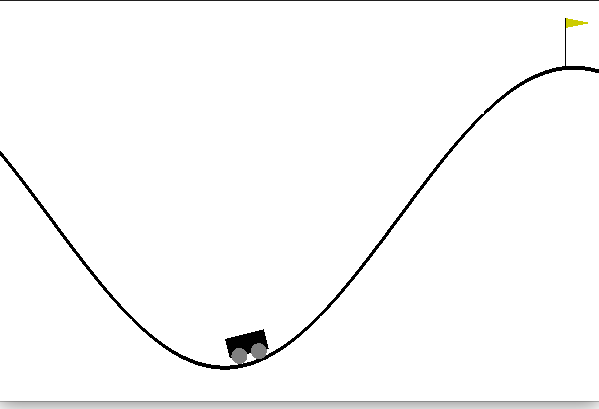
\includegraphics[scale=0.5]{MoutainCar.png}
\end{center}

This is a simple environment and is a great example to start with. It has a small state space, only position, and velocity of the car, which allows us to visualize the expert and learned policies. Below are some of the results.

\begin{table}[H]
\caption{Mountain Car Corrupted Data} % title of Table
\centering % used for centering table
    \begin{tabular}{c c} % centered columns (4 columns)
        \hline\hline %inserts double horizontal lines
        Metric &  Average Reward \\ [0.5ex] % inserts table
        %heading
        \hline % inserts single horizontal line
         Expert &  -103.9 $\pm$ 6.04
         \\ % inserting body of the table
        R-PIL & -104.45 $\pm$ 8.50   \\ % inserting body of the table
       LogReg & -132.0 $\pm$ 14.36\\
        \hline %inserts single line
    \end{tabular}
\label{MountainCarCorrupted} % is used to refer this table in the text
\end{table}

\begin{table}[H]
\caption{Mountain Car Random Policy} % title of Table
\centering % used for centering table
    \begin{tabular}{c c} % centered columns (4 columns)
        \hline\hline %inserts double horizontal lines
        Metric &  Average Reward \\ [0.5ex] % inserts table
        %heading
        \hline % inserts single horizontal line
         Expert &  -103.9 $\pm$ 6.04
         \\ % inserting body of the table
        R-PIL & -106.25 $\pm$ 6.00   \\ % inserting body of the table
       LogReg & -119.5 $\pm$ 1.75\\
        \hline %inserts single line
    \end{tabular}
\label{MountainCarRandom} % is used to refer this table in the text
\end{table}

\subsection{Lunar Lander}


\quad "Landing pad is always at coordinates (0,0). Coordinates are the first two numbers in state vector. Reward for moving from the top of the screen to landing pad and zero speed is about 100..140 points. If lander moves away from landing pad it loses reward back. Episode finishes if the lander crashes or comes to rest, receiving additional -100 or +100 points. Each leg ground contact is +10. Firing main engine is -0.3 points each frame. Solved is 200 points. Landing outside landing pad is possible. Fuel is infinite, so an agent can learn to fly and then land on its first attempt. Four discrete actions available: do nothing, fire left orientation engine, fire main engine, fire right orientation engine." \cite{brockman2016openai}


\begin{center}
    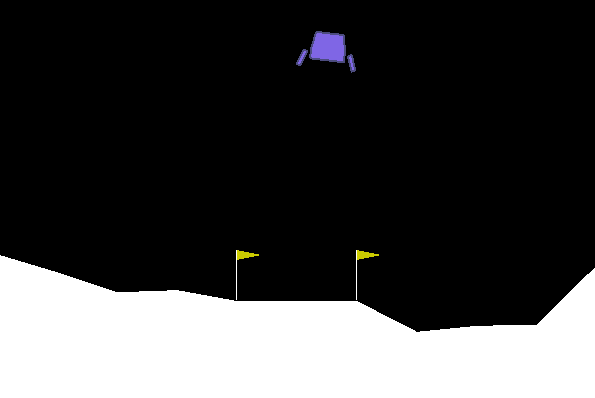
\includegraphics[scale=0.5]{LunarLander.png}
\end{center}
    
    
\begin{table}[H]
\caption{Lunar Lander Corrupted Data} % title of Table
\centering % used for centering table
    \begin{tabular}{c c} % centered columns (4 columns)
        \hline\hline %inserts double horizontal lines
        Metric &  Average Reward \\ [0.5ex] % inserts table
        %heading
        \hline % inserts single horizontal line
        Expert &  254.45 $\pm$ 57.09
         \\ % inserting body of the table
        R-PIL & 195.06 $\pm$ 64.45    \\ % inserting body of the table
      LogReg & -22.24 $\pm$ 48.51
      \\
        \hline %inserts single line
    \end{tabular}
\label{LunarLanderCorrupted} % is used to refer this table in the text
\end{table}

\begin{table}[H]
\caption{Lunar Lander Random Policy} % title of Table
\centering % used for centering table
    \begin{tabular}{c c} % centered columns (4 columns)
        \hline\hline %inserts double horizontal lines
        Metric &  Average Reward \\ [0.5ex] % inserts table
        %heading
        \hline % inserts single horizontal line
        Expert &  254.45 $\pm$ 57.09
         \\ % inserting body of the table
        R-PIL & 226.49 $\pm$ 49.52   \\ % inserting body of the table
       LogReg & -342.64 $\pm$ 35.53\\
        \hline %inserts single line
    \end{tabular}
\label{LunarLanderRandom} % is used to refer this table in the text
\end{table}

\subsection{Acrobot}

\quad "The acrobot system includes two joints and two links, where the joint between the two links is actuated. Initially, the links are hanging downwards, and the goal is to swing the end of the lower link up to a given height." \cite{brockman2016openai}
 
 
\begin{center}
    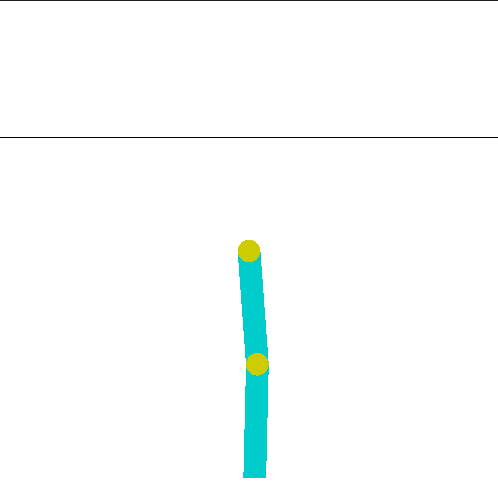
\includegraphics[scale=0.5]{Acrobot.png}
\end{center}

 \begin{table}[H]
\caption{Acrobot Corrupted Data} % title of Table
\centering % used for centering table
    \begin{tabular}{c c} % centered columns (4 columns)
        \hline\hline %inserts double horizontal lines
        Metric &  Average Reward \\ [0.5ex] % inserts table
        %heading
        \hline % inserts single horizontal line
        Expert &  -80.65 $\pm$ 3.49
         \\ % inserting body of the table
         R-PIL & -102.7 $\pm$ 22.62     \\ % inserting body of the table
       LogReg & -102.05$\pm$ 31.67
       
      \\
        \hline %inserts single line
    \end{tabular}
\label{LunarLanderCorrupted} % is used to refer this table in the text
\end{table}

\begin{table}[H]
\caption{Acrobot Random Policy} % title of Table
\centering % used for centering table
    \begin{tabular}{c c} % centered columns (4 columns)
        \hline\hline %inserts double horizontal lines
        Metric &  Average Reward \\ [0.5ex] % inserts table
        %heading
        \hline % inserts single horizontal line
        Expert &  -80.65 $\pm$ 3.49
         \\ % inserting body of the table
        R-PIL & -92.85 $\pm$ 23.81   \\ % inserting body of the table
       LogReg & -397.65 $\pm$ 85.18\\
        \hline %inserts single line
    \end{tabular}
\label{LunarLanderRandom} % is used to refer this table in the text
\end{table}


\section{Future Work}

\quad Going forward with the project, it would be interesting to apply this to other frameworks. As the core of the contribution of this paper is in dealing with adversarial demonstrations through probabilistic re-weighting, this can be generalized to a number of different models. It would also be interesting to expand this concept to non-discrete action spaces. If these extensions are possible this method would be of great interest in the IL community.



\section{Citations}
 
\printbibliography 

\section{Apendix}

\begin{figure}[H]
    \centering
    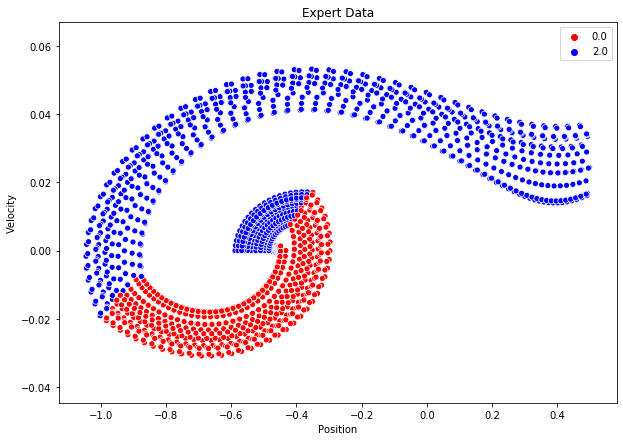
\includegraphics[scale=0.5]{ExpertData.png}
    \caption{20 Expert Demonstrations}
    \label{Expert Data}
\end{figure}

\begin{figure}[H]
    \centering
    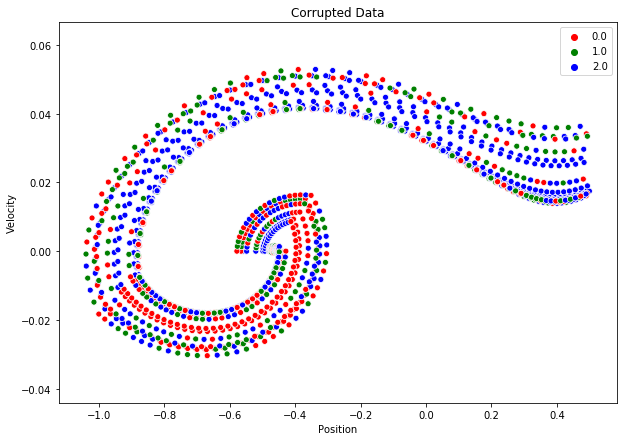
\includegraphics[scale=0.5]{CorruptedData.png}
    \caption{10 Expert demonstrations, 10 Corrupted Demonstrations}
    \label{CorruptedData}
\end{figure}

\begin{figure}[H]
    \centering
    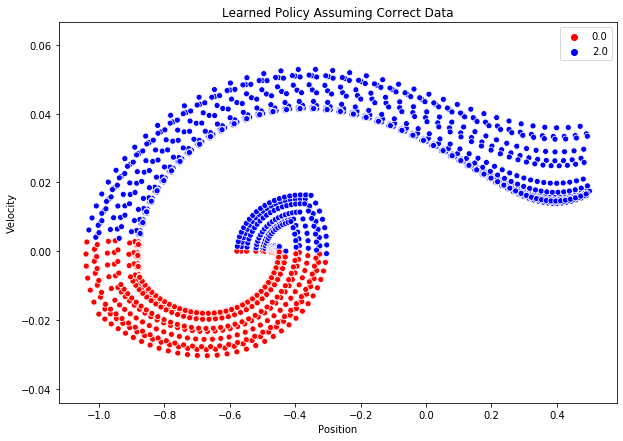
\includegraphics[scale=0.5]{LearnedPolicyBad.png}
    \caption{Learned policy assuming demonstrations are correct}
    \label{log_reg_corrupted}
\end{figure}

\begin{figure}[H]
    \centering
    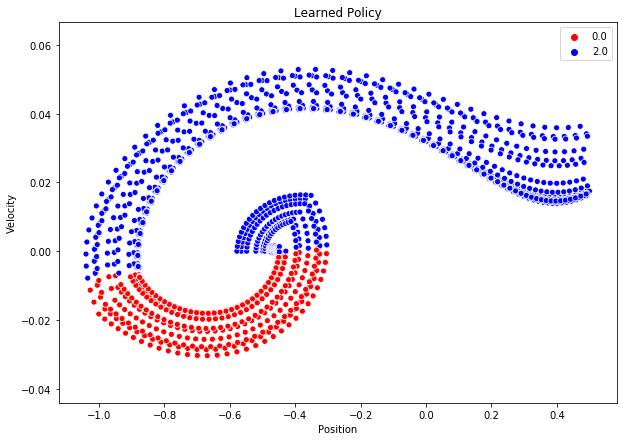
\includegraphics[scale=0.5]{LearnedPolicy.png}
    \caption{Learned policy R-PIL}
    \label{rpil_corrupted}
\end{figure}

\begin{figure}[H]
    \centering
    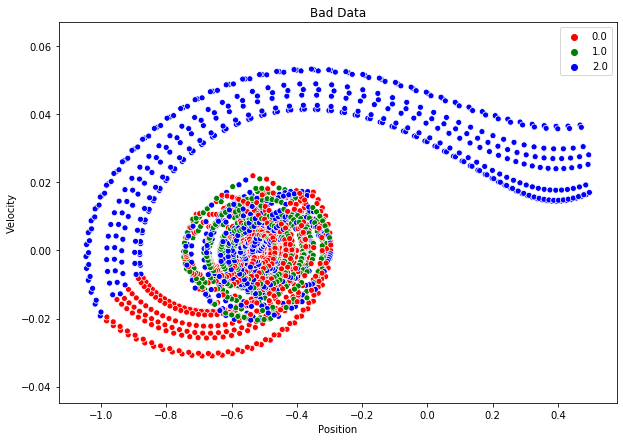
\includegraphics[scale=0.5]{RandomData.png}
    \caption{10 expert demonstrations, 10 demonstrations following a random policy}
    \label{RandomData}
\end{figure}

\begin{figure}[H]
    \centering
    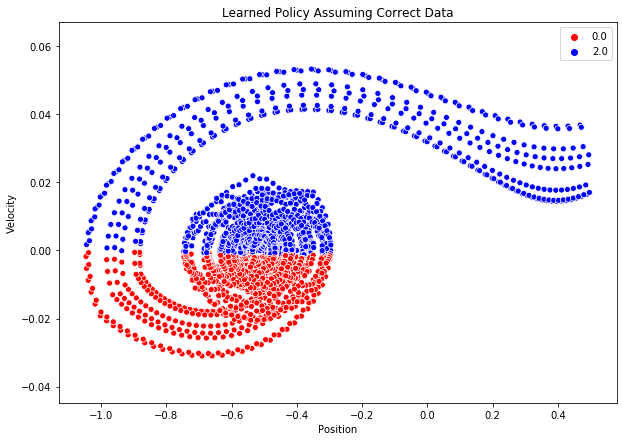
\includegraphics[scale=0.5]{LearnedPolicy2Bad.png}
    \caption{Learned policy assume demonstrations are correct}
    \label{log_reg_random}
\end{figure}

\begin{figure}[H]
    \centering
    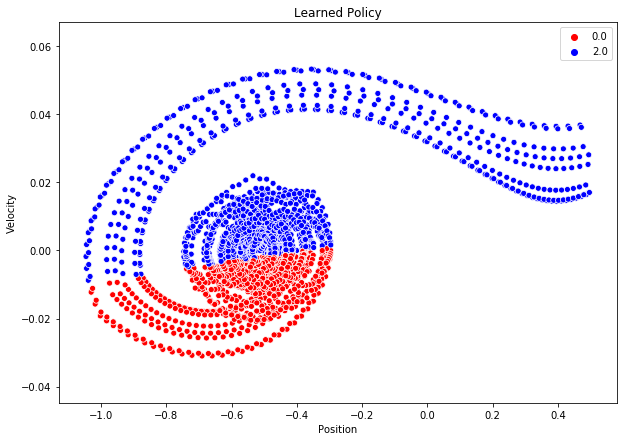
\includegraphics[scale=0.5]{LearnedPolicy2.png}
    \caption{Learned policy R-PIL}
    \label{rpil_random}
\end{figure}

\end{document}
